\documentclass[12pt,twoside]{article}

\textwidth 17cm \textheight 25cm \evensidemargin 0cm
\oddsidemargin 0cm \topmargin -2.5cm
\parindent 0pt
%\parskip \bigskipamount

\usepackage{graphicx}
\usepackage[dutch]{babel}
\usepackage{amssymb,amsthm,amsmath}
\usepackage[utf8]{inputenc}
\usepackage{nopageno}
\usepackage{pdfpages}
\usepackage{enumerate}
\usepackage{caption}
\usepackage{wrapfig}
\usepackage{pgf,tikz}
\usepackage{color}
\usetikzlibrary{arrows}
\usetikzlibrary{patterns}
\usepackage{fancyhdr}
\pagestyle{fancy}
\usepackage[version=3]{mhchem}
\usepackage{multicol}
\usepackage{fix-cm}
\usepackage{setspace}
\usepackage{mhchem}
\usepackage{xhfill}
\usepackage{parskip}
\usepackage{cancel}
\usepackage{mdframed}
\usepackage{url}

\newcommand{\todo}[1]{{\color{red} TODO: #1}}

\newcommand{\degree}{\ensuremath{^\circ}}
\newcommand\rad{\qopname\relax o{\mathrm{rad}}}

\newcommand\ggd{\qopname\relax o{\mathrm{ggd}}}

\def\LRA{\Leftrightarrow}%\mkern40mu}

\newcommand{\zrmbox}{\framebox{\phantom{EXE}}\phantom{X}}
\newcommand{\zrm}[1]{\framebox{#1}}

% environment oefening:
% houdt een teller bij die de oefeningen nummert, probeert ook de oefening op één pagina te houden
\newcounter{noefening}
\setcounter{noefening}{0}
\newenvironment{oefening}
{
  \stepcounter{noefening}
  \pagebreak[0]
  \begin{minipage}{\textwidth}
  \vspace*{0.7cm}{\large\bf Oefening \arabic{noefening}}
}{%
  \end{minipage}
}

\usepackage{calc}

% vraag
\reversemarginpar
\newcounter{punten}
\setcounter{punten}{0}
\newcounter{nvraag}
\setcounter{nvraag}{1}
\newlength{\puntwidth}
\newlength{\boxwidth}
\newcommand{\vraag}[1]{
\settowidth{\puntwidth}{\Large{#1}}
\setlength{\boxwidth}{1.5cm}
\addtolength{\boxwidth}{-\puntwidth}
{\large\bf Vraag \arabic{nvraag} \addtocounter{nvraag}{1}}\vspace*{-0.5cm}
{\marginpar{\color{lightgray}\fbox{\parbox{1.5cm}{\vspace*{1cm}\hspace*{\boxwidth}{\Large{#1}}}}}
\vspace*{0.5cm}}
\addtocounter{punten}{#1}}

% arulefill
\newcommand\arulefill[1][]{
  \ifstrempty{#1}{
    \leavevmode{
      \xrfill[-5pt]{0.3pt}[lightgray]
      \endgraf
    }
    \vspace*{0.2cm}
  }{
    \leavevmode{
      \xrfill[-5pt]{0.3pt}[lightgray]
      \endgraf
      \vspace*{0.2cm}
    }
    \foreach \n in {1,...,#1}{
      \leavevmode{
        \xrfill[-5pt]{0.3pt}[lightgray]
        \endgraf
        \vspace*{0.2cm}
      }
    }
  }
}
% \arules{n}
\newcommand{\arules}[1]{
\mbox{}
\color{lightgray}
%\vspace*{0.05cm}
\foreach \n in {1,...,#1}{
  \vspace*{0.75cm}
  \hrule height 0.3pt\hfill
}\color{black}\vspace*{0.2cm}}

% \arule{x}
\newcommand{\arule}[1]{
\color{lightgray}{\raisebox{-0.1cm}{\rule[-0.05cm]{#1}{0.3pt}}}\color{black}
}

% \abox{y}
\newcommand{\abox}[1]{
\fbox{
\begin{minipage}{\textwidth- 4\fboxsep}
\hspace*{\textwidth}\vspace{#1}
\end{minipage}
}
}

\newcommand{\ruitjes}[1]{
\definecolor{cqcqcq}{rgb}{0.85,0.85,0.85}
\hspace*{-2.5cm}
\begin{tikzpicture}[scale=1.04,line cap=round,line join=round,>=triangle 45,x=1.0cm,y=1.0cm]
\draw [color=cqcqcq, xstep=0.5cm, ystep=0.5cm] (0,-#1) grid (20.5,0);
\end{tikzpicture}
}


\newcommand{\assenstelsel}[5][1]{
\definecolor{cqcqcq}{rgb}{0.65,0.65,0.65}
\begin{tikzpicture}[scale=#1,line cap=round,line join=round,>=triangle 45,x=1.0cm,y=1.0cm]
\draw [color=cqcqcq,dash pattern=on 1pt off 1pt, xstep=1.0cm,ystep=1.0cm] (#2,#4) grid (#3,#5);
\draw[->,color=black] (#2,0) -- (#3,0);
\draw[shift={(1,0)},color=black] (0pt,2pt) -- (0pt,-2pt) node[below] {\footnotesize $1$};
\draw[color=black] (#3.25,0.07) node [anchor=south west] { x};
\draw[->,color=black] (0,#4) -- (0,#5);
\draw[shift={(0,1)},color=black] (2pt,0pt) -- (-2pt,0pt) node[left] {\footnotesize $1$};
\draw[color=black] (0.09,#5.25) node [anchor=west] { y};
\draw[color=black] (0pt,-10pt) node[right] {\footnotesize $0$};
\end{tikzpicture}
}

\newcommand{\getallenas}[3][1]{
\definecolor{cqcqcq}{rgb}{0.65,0.65,0.65}
\begin{tikzpicture}[scale=#1,line cap=round,line join=round,>=triangle 45,x=1.0cm,y=1.0cm]
\draw [color=cqcqcq,dash pattern=on 1pt off 1pt, xstep=1.0cm,ystep=1.0cm] (#2,-0.2) grid (#3,0.2);
\draw[->,color=black] (#2.25,0) -- (#3.5,0);
\draw[shift={(0,0)},color=black] (0pt,2pt) -- (0pt,-2pt) node[below] {\footnotesize $0$};
\draw[shift={(1,0)},color=black] (0pt,2pt) -- (0pt,-2pt) node[below] {\footnotesize $1$};
\draw[color=black] (#3.25,0.07) node [anchor=south west] {$\mathbb{R}$};
\end{tikzpicture}
}

\newcommand{\visgraad}[1]{\begin{tabular}{p{0.5cm}|p{#1}}&\\\hline\\\end{tabular}}

\newcommand{\tekenschema}[2]{\begin{tabular}{p{0.5cm}|p{#1}}&\\\hline\\[#2]\end{tabular}}

% schema van Horner
\newcommand{\schemahorner}{
\begin{tabular}{p{0.5cm}|p{7cm}}
&\\[1.5cm]
\hline\\
\end{tabular}}

% geef tabular iets meer ruimte
\setlength{\tabcolsep}{14pt}
\renewcommand{\arraystretch}{1.5}

\newcommand{\toets}[3]{
\thispagestyle{plain}
\vspace*{-2.5cm}
\begin{tikzpicture}[remember picture, overlay]
    \node [shift={(15.25 cm,-1.6cm)}] {%
        \includegraphics[width=1.8cm]{/home/ppareit/kaa1415/logokaavelgem.png}%
    };%
\end{tikzpicture}

\begin{tabular}{|llc|c|}
\hline
\vspace*{-0.5cm}
&&&\\
Naam & \arule{4cm} & {\Large\bf KA AVELGEM} & \\
\vspace*{-0.75cm}
&&&\\
Klas & \arule{4cm} & {\Large\bf 20...-...-...} & \\
\hline
\vspace*{-0.75cm}
&&&\\
Toets & {\bf #2} & {\large\bf #1} & Beoordeling\\
\vspace*{-0.75cm}
&&&\\
Onderwerp & \multicolumn{2}{l|}{\bf #3} &\\
\hline
\end{tabular}
}

\newcommand{\oefeningen}[1]{

\fancyhead[LE, RO]{\vspace{0.5cm} #1}
%\thispagestyle{plain}

{\bf \Large \centering Oefeningen: #1}

}

\raggedbottom

\newcommand\dom{\qopname\relax o{\mathrm{dom}}}
\newcommand\ber{\qopname\relax o{\mathrm{ber}}}

\newcommand\mC{\qopname\relax o{\mathrm{mC}}}
\newcommand\uC{\qopname\relax o{\mathrm{{\mu}C}}}
\newcommand\C{\qopname\relax o{\mathrm{C}}}

\newcommand\W{\qopname\relax o{\mathrm{W}}}
\newcommand\kW{\qopname\relax o{\mathrm{kW}}}
\newcommand\kWh{\qopname\relax o{\mathrm{kWh}}}


\newcommand\V{\qopname\relax o{\mathrm{V}}}
\newcommand\ohm{\qopname\relax o{\mathrm{\Omega}}}
\newcommand\kohm{\qopname\relax o{\mathrm{k\Omega}}}


\newcommand\N{\qopname\relax o{\mathrm{N}}}

\newcommand\Nperkg{\qopname\relax o{\mathrm{N/kg}}}

\newcommand\Nperm{\qopname\relax o{\mathrm{N/m}}}

\newcommand\gpermol{\qopname\relax o{\mathrm{g/mol}}}


\newcommand\kgperm{\qopname\relax o{\mathrm{kg/m}}}
\newcommand\kgperdm{\qopname\relax o{\mathrm{kg/dm}}}
\newcommand\gpercm{\qopname\relax o{\mathrm{g/cm}}}
\newcommand\gperml{\qopname\relax o{\mathrm{g/ml}}}


\newcommand{\mA}{\;\mbox{mA}}
\newcommand{\A}{\;\mbox{A}}
\newcommand{\MA}{\;\mbox{MA}}

\newcommand{\us}{\;\mu\mbox{s}}
\newcommand\s{\qopname\relax o{\mathrm{s}}}

\newcommand\h{\qopname\relax o{\mathrm{h}}}

\newcommand{\mpers}{\;\mbox{m/s}}
\newcommand{\kmperh}{\;\mbox{km/h}}
\newcommand{\kmpermin}{\;\mbox{km/min}}
\newcommand{\kmpers}{\;\mbox{km/s}}

\newcommand{\mph}{\;\mbox{mph}}

\newcommand{\Hz}{\;\mbox{Hz}}

\newcommand\Gm{\qopname\relax o{\mathrm{Gm}}}
\newcommand\Mm{\qopname\relax o{\mathrm{Mm}}}
\newcommand\km{\qopname\relax o{\mathrm{km}}}
\newcommand\hm{\qopname\relax o{\mathrm{hm}}}
\newcommand\dam{\qopname\relax o{\mathrm{dam}}}
\newcommand\m{\qopname\relax o{\mathrm{m}}}
\newcommand\dm{\qopname\relax o{\mathrm{dm}}}
\newcommand\cm{\qopname\relax o{\mathrm{cm}}}
\newcommand\mm{\qopname\relax o{\mathrm{mm}}}
\newcommand\um{\qopname\relax o{\mathrm{{\mu}m}}}
\newcommand\nm{\qopname\relax o{\mathrm{nm}}}


\newcommand\Gg{\qopname\relax o{\mathrm{Gg}}}
\newcommand\Mg{\qopname\relax o{\mathrm{Mg}}}
\newcommand\kg{\qopname\relax o{\mathrm{kg}}}
\newcommand\hg{\qopname\relax o{\mathrm{hg}}}
\renewcommand\dag{\qopname\relax o{\mathrm{dag}}}
\newcommand\g{\qopname\relax o{\mathrm{g}}}
\newcommand\dg{\qopname\relax o{\mathrm{dg}}}
\newcommand\cg{\qopname\relax o{\mathrm{cg}}}
\newcommand\mg{\qopname\relax o{\mathrm{mg}}}
\newcommand\ug{\qopname\relax o{\mathrm{{\mu}g}}}
\renewcommand\ng{\qopname\relax o{\mathrm{ng}}}

\newcommand\ton{\qopname\relax o{\mathrm{ton}}}

\newcommand\Gl{\qopname\relax o{\mathrm{Gl}}}
\newcommand\Ml{\qopname\relax o{\mathrm{Ml}}}
\newcommand\kl{\qopname\relax o{\mathrm{kl}}}
\newcommand\hl{\qopname\relax o{\mathrm{hl}}}
\newcommand\dal{\qopname\relax o{\mathrm{dal}}}
\renewcommand\l{\qopname\relax o{\mathrm{l}}}
\newcommand\dl{\qopname\relax o{\mathrm{dl}}}
\newcommand\cl{\qopname\relax o{\mathrm{cl}}}
\newcommand\ml{\qopname\relax o{\mathrm{ml}}}
\newcommand\ul{\qopname\relax o{\mathrm{{\mu}l}}}
\newcommand\nl{\qopname\relax o{\mathrm{nl}}}

\newcommand\MJ{\qopname\relax o{\mathrm{MJ}}}
\newcommand\kJ{\qopname\relax o{\mathrm{kJ}}}
\newcommand\J{\qopname\relax o{\mathrm{J}}}

\newcommand\T{\qopname\relax o{\mathrm{T}}}
\newcommand\uT{\qopname\relax o{\mathrm{{\mu}T}}}

\newcommand\grC{\qopname\relax o{\mathrm{{\degree}C}}}

\newcommand\K{\qopname\relax o{\mathrm{K}}}
\newcommand\calperK{\qopname\relax o{\mathrm{cal/K}}}

\newcommand\hPa{\qopname\relax o{\mathrm{hPa}}}
\newcommand\Pa{\qopname\relax o{\mathrm{Pa}}}

\newcommand\dB{\qopname\relax o{\mathrm{dB}}}

\newcommand{\EE}[1]{\cdot 10^{#1}}

\onehalfspacing

%\singlespacing
%\onehalfspacing
%\doublespacing

%\setlength{\headsep}{0cm}

\newenvironment{exlist}[1] %
{ \begin{multicols}{#1}
  \begin{enumerate}[(a)]
    \setlength{\itemsep}{0.8em} }
{ \end{enumerate}
  \end{multicols} }




\usepackage{pgfplots}

%\renewcommand{\rmdefault}{phv} % Arial
%\renewcommand{\sfdefault}{phv} % Arial

\begin{document}

\thispagestyle{empty}
\begin{center}
  \begin{mdframed}
  \centering
  \fontsize{50}{70}\selectfont De normale verdeling
  \end{mdframed}
  \vfill
  
\includegraphics[width=0.8\textwidth]{normal}
  \vfill
\end{center}
%\vfill
\vspace*{-2cm}
\subsection*{Doelstellingen}
{\singlespacing
Je \hfill  {\scriptsize(LP 2005/069, LI 2.3.2, ET16)}
\begin{itemize}
  \item kan aan de hand van voorbeelden, in betekenisvolle situaties, gebruik maken van de normale verdeling (met de bijhorende klokcurve) als model van een reeks statistische gegevens.
  \item kan het gemiddelde en de standaardafwijking gebruiken als karakteristieken van een normale verdeling en deze kengetallen ook grafisch interpreteren.
\end{itemize}

\thispagestyle{empty}
\mbox{}
\newpage
\clearpage
\thispagestyle{empty}
\tableofcontents
\newpage
\clearpage
\pagenumbering{arabic} 

\fancyhead[RO,LE]{De normale verdeling}
\fancyhead[RE,LO]{}

\onehalfspacing

\section{Inleiding}

Vorig jaar heeft een bekend kledingmerk een statistische onderzoek verricht naar de lichaamsafmetingen van vrouwen. Dit om beter passende kledij te ontwikkelen. Voor het onderzoek werden bij 160 willekeurig gekozen vrouwen 11 lichamelijke kenmerken gemeten. De resultaten voor de lichaamslengte vind je in onderstaande dataset:

\begin{center}  
\singlespacing
\scriptsize
166.38
165.46
163.8
169.75
168.27
167.44
165.56
165.75
166.13
165.41
168.69
166.14
166.68
165.99
164.67
164.26
165.05
168.58
166.6
168.13
161.26
167.9
165.5
164.28
163.38
167.01
164.52
162.84
166.19
165.3
167.28
165.32
167.57
168.4
163.71
166.59
167.85
164.36
166.83
166.05
163.94
164.85
168
166.2
167.14
162.93
169.47
166.84
169.08
166.58
166.53
165.85
167.04
168.66
169.41
170.1
164.27
163.26
164.8
164.49
164.54
169.09
165.39
164.29
164.86
166.14
166.49
167.32
164.38
166.54
170.92
163.83
167.41
168.67
168.88
167.66
165.89
166.17
165.4
166.27
166.32
162.55
169.33
168.61
167.09
164.28
165.94
164.22
165.43
164.07
167.75
163.86
167.35
163.78
167.08
167.82
164.48
166.06
164.62
167.08
169.12
166.27
163.5
168.67
164.44
165.63
164.62
165.56
166.86
164.41
166.95
167.41
167.43
166.06
166.73
168.92
167.56
168.81
166.89
164.34
164.3
165.24
168.7
165.63
164.34
165.41
165.71
165.58
166.49
165.61
167.36
169.06
164.41
167.77
167.16
168.1
164.56
162.29
166.1
164.13
159.48
167.98
162.43
167.57
167.25
163.9
168.06
160.94
164.24
163.75
168.11
162.9
164.1
165.36
165.81
166.31
163.96
166.32
165.45
165.06
\end{center}

Deze gegevens zeggen uiteraard niet veel. Omdat de gegevens \arule{4cm} zijn, verdelen we ze in 10 klassen en plaatsen we ze in volgende \arule{4cm}:

\begin{center}
\definecolor{cqcqcq}{rgb}{0.75,0.75,0.75}
\begin{tikzpicture}[yscale=0.2, line cap=round,line join=round,>=triangle 45,x=1.0cm,y=1.0cm]
\draw [color=cqcqcq,dash pattern=on 7pt off 7pt, xstep=2.0cm,ystep=10.0cm] (159.01,-4.38) grid (171.44,44.53);
\draw[->,color=black] (159.01,0) -- (171.44,0);
\foreach \x in {160,162,164,166,168,170}
\draw[shift={(\x,0)},color=black] (0pt,2pt) -- (0pt,-2pt) node[below] {\footnotesize $\x$};
\clip(159.01,-4.38) rectangle (171.44,44.53);
\draw[line width=1.2pt,fill=black,fill opacity=0.3] (159.48,0) rectangle (160.63,1);
\draw[line width=1.2pt,fill=black,fill opacity=0.3] (160.63,0) rectangle (161.77,2);
\draw[line width=1.2pt,fill=black,fill opacity=0.3] (161.77,0) rectangle (162.91,5);
\draw[line width=1.2pt,fill=black,fill opacity=0.3] (162.91,0) rectangle (164.06,13);
\draw[line width=1.2pt,fill=black,fill opacity=0.3] (164.06,0) rectangle (165.2,31);
\draw[line width=1.2pt,fill=black,fill opacity=0.3] (165.2,0) rectangle (166.35,40);
\draw[line width=1.2pt,fill=black,fill opacity=0.3] (166.35,0) rectangle (167.49,31);
\draw[line width=1.2pt,fill=black,fill opacity=0.3] (167.49,0) rectangle (168.63,19);
\draw[line width=1.2pt,fill=black,fill opacity=0.3] (168.63,0) rectangle (169.78,16);
\draw[line width=1.2pt,fill=black,fill opacity=0.3] (169.78,0) rectangle (170.92,2);
\end{tikzpicture}
\end{center}

\begin{minipage}{\textwidth}
We laten {\em GeoGebra} ook de volgende \arule{4cm} uitrekenen, we vinden volgende resultaten:

%\begin{center}
  \begin{tabular}{c l|r}
      \arule{4cm} & $n$ & 160\\
      \arule{4cm} & $\bar{x}$ & 166.03\\
      \arule{4cm} & $s$ & 1.94\\
                    & min & 159.5\\
                    & $Q_1$ & 164.5\\
                    & Med & 166.07\\
                    & $Q_3$ & 167.4\\
                    & max & 170.9\\
  \end{tabular}
%\end{center}
\end{minipage}

Het histogram geeft ons de mogelijkheid een tweede grafiek te tekenen, de {\bf frequentiepolygoon}. Deze verkrijgen we door de middens van de bovenste zijden van alle rechthoeken met elkaar te verbinden.

\begin{oefening}
Teken op het bovenstaand histogram het frequentiepolygoon.
\end{oefening}

De ontstane kromme is een {\bf klokvormige kromme}, met een symmetrieas door het gemiddelde. Hoe hoger het aantal klassen, hoe vloeiender de kromme wordt. In de volgende figuur werd dit gedaan in de limiet (er werd aangenomen dat het onderzoek bij oneindig veel vrouwen werd uitgevoerd):

\begin{center}
\definecolor{cqcqcq}{rgb}{0.75,0.75,0.75}
\begin{tikzpicture}[yscale=0.2, line cap=round,line join=round,>=triangle 45,x=1.0cm,y=1.0cm]
\draw [color=cqcqcq,dash pattern=on 7pt off 7pt, xstep=2.0cm,ystep=10.0cm] (159.01,-4.38) grid (171.44,30.53);
\draw[->,color=black] (159.01,0) -- (171.44,0);
\foreach \x in {160,162,164,166,168,170}
\draw[shift={(\x,0)},color=black] (0pt,2pt) -- (0pt,-2pt) node[below] {\footnotesize $\x$};
\clip(159.01,-4.38) rectangle (171.44,32);
\draw[line width=1.6pt, smooth,samples=100,domain=150:176] plot(\x,{160*exp((-(((\x)-166)/2.05)^2)/2)/(sqrt(2*3.14)*abs(2.05))});
\end{tikzpicture}
\end{center}

\begin{oefening}
Waar ligt de symmetrieas in ons voorbeeld? \arule{4cm} Teken deze op bovenstaande grafiek.
\end{oefening}

Dit is een typisch voorbeeld van een {\bf normale verdeling}. Dergelijke kromme kan beschreven worden door een functie $f(x)$ die in de context van de statistiek een {\bf dichtheidsfunctie} genoemd word. In ons voorbeeld wordt het functievoorschrift

$$f(x)=\dfrac{1}{1.94\sqrt{2\pi}}\;e^{-\dfrac{1}{2}\left(\dfrac{x-166.03}{1.94}\right)^2}\;.$$

\pagebreak
\section{Algemeen}

\begin{minipage}{0.5\textwidth}
De grafieken van gegevens die een normale verdeling hebben, zijn steeds
\begin{itemize}
  \item symmetrische
  \item ééntoppige
  \item klokvormige
\end{itemize}
krommen. Ze hebben allemaal dezelfde globale vorm, zie rechts.
\end{minipage}
\begin{minipage}{0.5\textwidth}
\begin{center}
\definecolor{cqcqcq}{rgb}{0.75,0.75,0.75}
\begin{tikzpicture}[yscale=8, line cap=round,line join=round,>=triangle 45,x=1.0cm,y=1.0cm]
\draw [color=cqcqcq,dash pattern=on 1pt off 1pt, xstep=0.5cm,ystep=0.2cm] (-3.4,-0.1) grid (3.4,0.65);
\draw[->,color=black] (-3.5,0) -- (3.5,0);
\foreach \x in {-3,-2,-1,1,2,3}
\draw[shift={(\x,0)},color=black] (0pt,2pt) -- (0pt,-2pt) node[below] {\footnotesize $\x$};
\draw[->,color=black] (0,-0.1) -- (0,0.65);
\foreach \y in {0.2,0.4,0.6}
\draw[shift={(0,\y)},color=black] (2pt,0pt) -- (-2pt,0pt) node[left] {\footnotesize $\y$};
\clip(-3.5,-0.1) rectangle (3.5,0.65);
\draw[line width=1.6pt, smooth,samples=100,domain=-3.5:3.5] plot(\x,{exp((-((\x))^2)/2)/(sqrt(2*3.1415926535))});
\end{tikzpicture}
\end{center}
\end{minipage}

Vergelijk nu het voorschrift van $f(x)$ uit ons initieel voorbeeld, dat waarbij de lengtes van 160 dames werd gemeten, met de centrumgetallen en de spreidingsmaten van dat voorbeeld om een algemeen voorschrift af te leiden voor een normale verdeling:

\begin{oefening}
Vul de normale verdeling aan met $\bar{x}$ en $s$

$$f(x)=\dfrac{1}{\arule{1cm}{\sqrt{2\pi}}}\;e^{-\dfrac{1}{2}\left(\dfrac{x-\arule{1cm}}{\arule{1cm}}\right)^2}\;.$$
\end{oefening}

Wanneer een enquête wordt uitgevoerd, wordt steeds gewerkt met een steekproef. Voor deze steekproef berekenen we dan het gemiddelde $\bar{x}$ en de standaardafwijking $s$.

\begin{oefening}
Een steekproef wordt steeds genomen als een klein deel uit de \arule{5cm}. Waarom doen we dit?
\arules{3}
\end{oefening}

Indien de omvang van de steekproef voldoende groot is, veralgemenen we deze resultaten voor de volledige populatie. De populatie heeft echter zelf ook een gemiddelde en een standaardafwijking. Die kunnen lichtjes verschillen van deze van de steekproef. Om de twee niet te verwarren wordt een andere notatie toegekend:

\begin{center}
\begin{tabular}{c|c|c}
& Steekproef & Populatie\\
\hline
Gemiddelde & $\bar{x}$ & $\mu$ (mu)\\
Standaardafwijking & $s$ & $\sigma$ (sigma)\\
\end{tabular}
\end{center}

Zo wordt het algemene voorschrift voor een normaal verdeelde populatie:

$$f(x)=\dfrac{1}{\sigma{\sqrt{2\pi}}}\;e^{-\dfrac{1}{2}\left(\dfrac{x-\mu}{\sigma}\right)^2}$$

Omdat dit voorschrift volledig bepaald is door het gemiddelde $\mu$ en de standaardafwijking $\sigma$, noteren we dit kort als $N(\mu,\sigma)$.

\pagebreak
\section{Voorbeelden van normaal verdeelde gegevens}

De normale verdeling is zonder twijfel de meest gebruikte verdeling in de statistiek. Van heel wat gegevens is immers geweten dat ze normaal verdeeld zijn:
\begin{itemize}
  \item lengte en gewicht van mensen en dieren
  \item het IQ
  \item de effectieve inhoud van machinaal gevulde verpakkingen
  \item sportprestaties
\end{itemize}
\begin{oefening} Geef zelf een voorbeeld van normaal verdeelde gegevens:
\begin{itemize}
  \item \dotfill
\end{itemize}
\end{oefening}

Men mag hier echter niet uit besluiten dat alles normaal verdeeld zou zijn. Typische voorbeelden van niet-normaal verdeelde gegevens zijn:
\begin{itemize}
  \item de leeftijd bij het overlijden van mens of dier
  \item het inkomen
\end{itemize}
\begin{oefening} Geef zelf een voorbeeld van niet normaal verdeelde gegevens:
\begin{itemize}
  \item \dotfill
\end{itemize}
\end{oefening}

\begin{center}
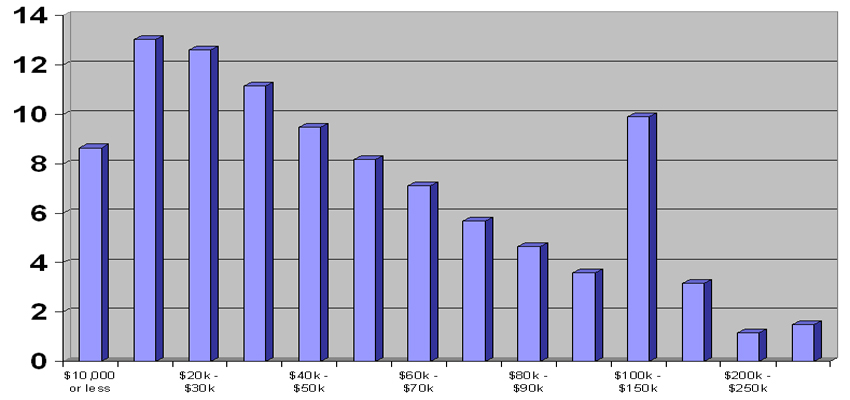
\includegraphics[width=\textwidth]{Income-curve}
\end{center}

\newpage
\section{Grafische betekenis van $\mu$ en $\sigma$}

\subsection{Grafische betekenis van $\mu$}

We laten in het functievoorschrift van de normale verdeling
$$f(x)=\dfrac{1}{\sigma{\sqrt{2\pi}}}\;e^{-\dfrac{1}{2}\left(\dfrac{x-\mu}{\sigma}\right)^2}$$
het gemiddelde $\mu$ variëren, terwijl de standaardafwijking $\sigma$ constant houden ($\sigma=1$). Hieronder zie je de grafieken voor verschillende waarden van $\mu$:
\begin{center}
\definecolor{cqcqcq}{rgb}{0.75,0.75,0.75}
\begin{tikzpicture}[yscale=8,line cap=round,line join=round,>=triangle 45,x=1.0cm,y=1.0cm]
\draw [color=cqcqcq,dash pattern=on 1pt off 1pt, xstep=1.0cm,ystep=0.1cm] (-6,-0.1) grid (6,0.6);
\draw[->,color=black] (-6,0) -- (6,0);
\foreach \x in {-6,-5,-4,-3,-2,-1,1,2,3,4,5}
\draw[shift={(\x,0)},color=black] (0pt,2pt) -- (0pt,-2pt) node[below] {\footnotesize $\x$};
\draw[->,color=black] (0,-0.1) -- (0,0.6);
\foreach \y in {,0.2,0.3,0.4,0.5}
\draw[shift={(0,\y)},color=black] (2pt,0pt) -- (-2pt,0pt) node[left] {\footnotesize $\y$};
\clip(-6,-0.1) rectangle (6,0.6);
\draw[line width=1.6pt, smooth,samples=100,domain=-6.0:6.0] plot(\x,{exp((-((\x))^2)/2)/(sqrt(2*3.1415926535)*abs(1))});
\draw[line width=1.6pt, smooth,samples=100,domain=-6.0:6.0] plot(\x,{exp((-((\x)+3)^2)/2)/(sqrt(2*3.1415926535)*abs(1))});
\draw[line width=1.6pt, smooth,samples=100,domain=-6.0:6.0] plot(\x,{exp((-((\x)-2)^2)/2)/(sqrt(2*3.1415926535)*abs(1))});
\draw (-5.5,0.38) node[anchor=north west] {$\mu=-3$};
\draw (0.3,0.5) node[anchor=north west] {$\mu=0$};
\draw (2.82,0.35) node[anchor=north west] {$\mu=2$};
\end{tikzpicture}
\end{center}

We merken dat de grafieken van al deze normale verdelingen met constante $\sigma=1$ op een verschuiving evenwijdig met de $x$-as met $\mu$ eenheden na gelijk zijn.

\begin{oefening}
Voor welke $x$-waarde vinden we steeds de top van de klokvormige kromme?
\arules{1}
\end{oefening}

\subsection{Grafische betekenis van $\sigma$}

We laten nu in het functievoorschrift 
$$f(x)=\dfrac{1}{\sigma{\sqrt{2\pi}}}\;e^{-\dfrac{1}{2}\left(\dfrac{x-\mu}{\sigma}\right)^2}$$
de standaardafwijking $\sigma$ variëren, terwijl we het gemiddelde $\mu$ constant houden op $\mu=0$.

\begin{center}
\definecolor{cqcqcq}{rgb}{0.75,0.75,0.75}
\begin{tikzpicture}[yscale=8, line cap=round,line join=round,>=triangle 45,x=1.0cm,y=1.0cm]
\draw [color=cqcqcq,dash pattern=on 1pt off 1pt, xstep=2.0cm,ystep=0.2cm] (-5.5,-0.1) grid (5.5,0.85);
\draw[->,color=black] (-6,0) -- (7,0);
\foreach \x in {-6,-4,-2,2,4,6}
\draw[shift={(\x,0)},color=black] (0pt,2pt) -- (0pt,-2pt) node[below] {\footnotesize $\x$};
\draw[->,color=black] (0,-0.1) -- (0,0.9);
\foreach \y in {,0.2,0.4,0.6,0.8}
\draw[shift={(0,\y)},color=black] (2pt,0pt) -- (-2pt,0pt) node[left] {\footnotesize $\y$};
\clip(-6,-0.1) rectangle (6,0.85);
\draw[line width=1.6pt, smooth,samples=100,domain=-6.0:6.0] plot(\x,{exp((-((\x))^2)/2)/(sqrt(2*3.1415926535)*abs(1))});
\draw[line width=1.6pt, smooth,samples=100,domain=-6.0:6.0] plot(\x,{exp((-(((\x))/0.5)^2)/2)/(sqrt(2*3.1415926535)*abs(0.5))});
\draw[line width=1.6pt, smooth,samples=100,domain=-6.0:6.0] plot(\x,{exp((-(((\x))/2)^2)/2)/(sqrt(2*3.1415926535)*abs(2))});
\draw[line width=1.6pt, smooth,samples=100,domain=-6.0:6.0] plot(\x,{exp((-(((\x))/4)^2)/2)/(sqrt(2*3.1415926535)*abs(4))});
\draw (0.6,0.76) node[anchor=north west] {$\sigma=0.5$};
\draw (1.0,0.35) node[anchor=north west] {$\sigma=1$};
\draw (1.7,0.22) node[anchor=north west] {$\sigma=2$};
\draw (4,0.13) node[anchor=north west] {$\sigma=4$};
\end{tikzpicture}
\end{center}

We merken dat de grafieken van al deze normale verdelingen met constante $\mu=0$ qua vorm gelijk zijn. Ze hebben wel allemaal een uitrekking of inkrimping evenwijdig met de \arule{2cm} ondergaan.

\begin{oefening}
Vul volgende tabel aan:
\begin{center}
  \begin{tabular}{c|c}
    $\sigma$ & Hoogte van de top\\
    \hline
    0.5 & \arule{2cm}\\
    1 & \arule{2cm}\\
    2 & \arule{2cm}\\
    4 & \arule{2cm}
  \end{tabular}
\end{center}
\end{oefening}

\begin{oefening}
Probeer in te schatten waar de top zou liggen als $\sigma=0.25$ zou zijn?
\arules{1}
\end{oefening}

Besluit: De hoogte van de top is \dotfill

De waarde van $\sigma$ geeft aan of de curve breed (bij een \arule{4cm} standaardafwijking) of spits (bij een \arule{4cm} standaardafwijking) is.

\begin{oefening}
Bepaal in de onderstaande grafieken het gemiddelde $\mu$ en de standaardafwijking $\sigma$ van de vet gedrukte functie.

\definecolor{cqcqcq}{rgb}{0.75,0.75,0.75}
\begin{multicols}{2}
\begin{center}
\begin{tikzpicture}[xscale=0.6,yscale=5,line cap=round,line join=round,>=triangle 45,x=1.0cm,y=1.0cm]
\draw [color=cqcqcq,dash pattern=on 1pt off 1pt, xstep=2.0cm,ystep=0.2cm] (-5.9,-0.1) grid (5.9,0.9);
\draw[->,color=black] (-6,0) -- (6,0);
\foreach \x in {-4,-2,2,4}
\draw[shift={(\x,0)},color=black] (0pt,2pt) -- (0pt,-2pt) node[below] {\footnotesize $\x$};
\draw[->,color=black] (0,-0.1) -- (0,1);
\foreach \y in {,0.2,0.4,0.6,0.8}
\draw[shift={(0,\y)},color=black] (2pt,0pt) -- (-2pt,0pt) node[left] {\footnotesize $\y$};
\clip(-6,-0.1) rectangle (6,1);
\draw[line width=1.2pt, smooth,samples=100,domain=-6.0:6.0] plot(\x,{exp((-((\x))^2)/2)/(sqrt(2*3.1415926535)*abs(1))});
\draw[line width=2pt, smooth,samples=100,domain=-6.0:6.0] plot(\x,{exp((-(((\x)-3)/0.5)^2)/2)/(sqrt(2*3.1415926535)*abs(0.5))});
\end{tikzpicture}
$$\mu=\arule{1cm} \sigma=\arule{1cm}$$
\end{center}

\begin{center}
\begin{tikzpicture}[xscale=0.6,yscale=5,line cap=round,line join=round,>=triangle 45,x=1.0cm,y=1.0cm]
\draw [color=cqcqcq,dash pattern=on 1pt off 1pt, xstep=2.0cm,ystep=0.2cm] (-5.9,-0.1) grid (5.9,0.9);
\draw[->,color=black] (-6,0) -- (6,0);
\foreach \x in {-4,-2,2,4}
\draw[shift={(\x,0)},color=black] (0pt,2pt) -- (0pt,-2pt) node[below] {\footnotesize $\x$};
\draw[->,color=black] (0,-0.1) -- (0,1);
\foreach \y in {,0.2,0.4,0.6,0.8}
\draw[shift={(0,\y)},color=black] (2pt,0pt) -- (-2pt,0pt) node[left] {\footnotesize $\y$};
\clip(-6,-0.1) rectangle (6,1);
\draw[line width=1.2pt, smooth,samples=100,domain=-6.0:6.0] plot(\x,{exp((-((\x))^2)/2)/(sqrt(2*3.1415926535)*abs(1))});
\draw[line width=2pt, smooth,samples=100,domain=-6.0:6.0] plot(\x,{exp((-(((\x)+2)/2)^2)/2)/(sqrt(2*3.1415926535)*abs(2))});
\end{tikzpicture}
$$\mu=\arule{1cm} \sigma=\arule{1cm}$$
\end{center}

\begin{center}
\begin{tikzpicture}[xscale=0.6,yscale=5,line cap=round,line join=round,>=triangle 45,x=1.0cm,y=1.0cm]
\draw [color=cqcqcq,dash pattern=on 1pt off 1pt, xstep=2.0cm,ystep=0.2cm] (-5.9,-0.1) grid (5.9,0.9);
\draw[->,color=black] (-6,0) -- (6,0);
\foreach \x in {-4,-2,2,4}
\draw[shift={(\x,0)},color=black] (0pt,2pt) -- (0pt,-2pt) node[below] {\footnotesize $\x$};
\draw[->,color=black] (0,-0.1) -- (0,1);
\foreach \y in {,0.2,0.4,0.6,0.8}
\draw[shift={(0,\y)},color=black] (2pt,0pt) -- (-2pt,0pt) node[left] {\footnotesize $\y$};
\clip(-6,-0.1) rectangle (6,1);
\draw[line width=1.2pt, smooth,samples=100,domain=-6.0:6.0] plot(\x,{exp((-((\x))^2)/2)/(sqrt(2*3.1415926535)*abs(1))});
\draw[line width=2pt, smooth,samples=100,domain=-6.0:6.0] plot(\x,{exp((-(((\x)+3)/1)^2)/2)/(sqrt(2*3.1415926535)*abs(1))});
\end{tikzpicture}
$$\mu=\arule{1cm} \sigma=\arule{1cm}$$
\end{center}

\begin{center}
\begin{tikzpicture}[xscale=0.6,yscale=5,line cap=round,line join=round,>=triangle 45,x=1.0cm,y=1.0cm]
\draw [color=cqcqcq,dash pattern=on 1pt off 1pt, xstep=2.0cm,ystep=0.2cm] (-5.9,-0.1) grid (5.9,0.9);
\draw[->,color=black] (-6,0) -- (6,0);
\foreach \x in {-4,-2,2,4}
\draw[shift={(\x,0)},color=black] (0pt,2pt) -- (0pt,-2pt) node[below] {\footnotesize $\x$};
\draw[->,color=black] (0,-0.1) -- (0,1);
\foreach \y in {,0.2,0.4,0.6,0.8}
\draw[shift={(0,\y)},color=black] (2pt,0pt) -- (-2pt,0pt) node[left] {\footnotesize $\y$};
\clip(-6,-0.1) rectangle (6,1);
\draw[line width=1.2pt, smooth,samples=100,domain=-6.0:6.0] plot(\x,{exp((-((\x))^2)/2)/(sqrt(2*3.1415926535)*abs(1))});
\draw[line width=2pt, smooth,samples=100,domain=-6.0:6.0] plot(\x,{exp((-(((\x)-0)/4)^2)/2)/(sqrt(2*3.1415926535)*abs(4))});
\end{tikzpicture}
$$\mu=\arule{1cm} \sigma=\arule{1cm}$$
\end{center}
\end{multicols}
\end{oefening}

\pagebreak
\section{Standaardnormale kansverdeling}

In de vorige paragraaf werden grafieken van de normale verdeling verschoven (met behulp van $\mu$) en herschaald (met behulp van $\sigma$). Het is dus mogelijk om de normale verdeling te
\begin{itemize}
  \item verschuiven zodat het gemiddelde $\mu=0$ wordt,
  \item herschalen zodat de standaardafwijking $\sigma=1$ wordt.
\end{itemize}

Een normale verdelingen met gemiddelde 0 en standaardafwijking 1 of kort $N(0,1)$ noemen we {\bf standaardnormaal verdeeld}. Om aan te duiden dat we met de standaardnormale verdeling werken, gebruiken we de letter $Z$ i.p.v. $X$ om de kansvariabele aan te duiden.

Een normale verdeling herken je aan de grafiek van de kansfunctie. De grafiek is namelijk steeds een symmetrische, ééntoppige, klokvormige kromme. Op de volgende figuur zie je de grafiek horend bij N(0, 1).

\pgfmathdeclarefunction{gauss}{2}{%
  \pgfmathparse{1/(#2*sqrt(2*pi))*exp(-((x-#1)^2)/(2*#2^2))}%
}

\begin{center}
\begin{tikzpicture}
\begin{axis}[
  no markers, domain=0:10, samples=100,
  axis lines*=left, xlabel=$x$, ylabel=$f(x)$,
  every axis y label/.style={at={(0,1)},anchor=south},
  every axis x label/.style={at=(current axis.right of origin),anchor=west},
  height=8cm, width=16cm,
  xtick={-3,-2,-1,0,1,2,3}, ytick={0.1, 0.2, 0.3, 0.4},
  enlargelimits=false, clip=false, axis on top,
  grid = none
  ]
  \addplot [fill=gray!40, draw=none, domain=-1:1] {gauss(0,1)} \closedcycle;
  \addplot [very thick,black!50!black, domain=-4:4] {gauss(0,1)};
  \draw [yshift=-0.6cm] (axis cs:0,0) node[anchor=north] {$\mu$};
  \draw [yshift=-0.6cm] (axis cs:-1,0) node[anchor=north] {$-\sigma$};
  \draw [yshift=-0.6cm] (axis cs:1,0) node[anchor=north] {$\sigma$};
  \draw (axis cs:0,0.2) node[anchor=north] {$\pm 68.27\%$};
\end{axis}
\end{tikzpicture}
\end{center}

Voor de standaardnormale verdeling $N(0,1)$ worden de verdelingsfunctie $F(x)$, verwachtingswaarde $E(X)$ en standaardafwijking $\sigma$ gegeven door
\begin{itemize}
  \item $F(z)=P(Z\leq z)=\Phi(z)$ (zie verder)
  \item $E(Z)=\mu=0$
  \item $\sigma=1$
\end{itemize}

\subsection{Kansen berekenen bij standaardnormaal verdeelde populaties}

Om de kans te berekenen dat iemand minder heeft dan een bepaalde waarde, volstaat het om de oppervlakte onder de kromme te berekenen, zoals in onderstaande figuur:

\begin{center}
\begin{tikzpicture}
\begin{axis}[
  no markers, domain=0:10, samples=100,
  axis lines*=left, xlabel=$x$, ylabel=$f(x)$,
  every axis y label/.style={at={(0,1)},anchor=south},
  every axis x label/.style={at=(current axis.right of origin),anchor=west},
  height=8cm, width=16cm,
  xtick={0,1}, ytick={0.1, 0.2, 0.3, 0.4},
  enlargelimits=false, clip=false, axis on top,
  grid = none
  ]
  \addplot [fill=gray!40, draw=none, domain=-4:1.5] {gauss(0,1)} \closedcycle;
  \addplot [very thick,black!50!black, domain=-4:4] {gauss(0,1)};
  \draw [yshift=-0.1cm] (axis cs:1.5,0) node[anchor=north] {$z$};
  \draw (axis cs:0,0.2) node[anchor=north] {$\Phi(z)$};
\end{axis}
\end{tikzpicture}
\end{center}

De leerlingen die ook integraalrekenen krijgen zien onmiddellijk dat dit niets anders is dan de integraal
$$\Phi(z)=P(Z\leq z)=\dfrac{1}{\sqrt{2\pi}}\int_{-\infty}^{z}e^{-\frac{1}{2}t^2}dt\;.$$

Het berekenen van deze oppervlakteintegraal is vrij ingewikkeld. Voor de standaardnormale verdeling bestaat er echter een tabel waaruit je deze kansen rechtstreeks kan aflezen, zie bijlage.

\subsubsection*{Voorbeeld 1}

Gegeven: Een populatie die kan beschreven worden door een standaardnormale verdeling. Bereken het percentage waarnemingen kleiner dan $1.36$.

In symbolen: $\Phi(1.36)=P(Z\leq 1.36)$

Methode:
\begin{itemize}
  \item Zoek de waarde $1.36$ in de tabel.
  \begin{itemize}
    \item Voor de eerste 2 cijfers kijk je in de linkerkolom van de tabel: ga op zoek naar de rij die overeenstemt met de waarde 1.3.
    \item Vervolgens schuif je op naar rechts tot de kolom die overeenkomt met 0.06.
  \end{itemize}
  \item Het percentage waarnemingen kleiner dan 1.36 bedraagt dus 91.308\%
\end{itemize}

\begin{minipage}{0.5\textwidth}
$$\Phi(1.36)=P(Z\leq 1.36)=0.91308$$
$$\Rightarrow\Phi(1.36)=91.308\%$$
\end{minipage}
\begin{minipage}{0.5\textwidth}
\vspace*{0.8cm}
\begin{center}
\begin{tikzpicture}
\begin{axis}[
  no markers, domain=0:10, samples=100,
  axis lines*=left,
  height=4cm, width=8cm,
  xtick={1.36}, ytick={0}, yticklabels={},
  enlargelimits=false, clip=false, axis on top,
  grid = none
  ]
  \addplot [fill=gray!40, draw=none, domain=-4:1.36] {gauss(0,1)} \closedcycle;
  \addplot [very thick,black!50!black, domain=-4:4] {gauss(0,1)};
  \draw (axis cs:0,0.2) node[anchor=north] {$91\%$};
\end{axis}
\end{tikzpicture}
\end{center}
\end{minipage}

\subsubsection*{Voorbeeld 2}

Gegeven: Een populatie die kan beschreven worden door een standaardnormale verdeling. Bereken het percentage waarnemingen gelegen tussen $1.03$ en $2.95$.

In symbolen: $P(1.03\leq Z\leq 2.95)$

Dit is niet rechtstreeks in de tabel af te lezen. We herschrijven het gevraagde als volgt (zie figuur ter verduidelijking):

\begin{align*}
  P(1.03\leq Z\leq 2.95) &= P(Z\leq 2.95) - P(Z\leq 1.03)\\
                         &= \Phi(2.95) - \Phi(1.03)
\end{align*}

\begin{center}
\begin{tikzpicture}
\begin{axis}[
  no markers, domain=0:10, samples=100,
  axis lines*=left,
  height=6cm, width=14cm,
  xtick={1.03, 2.95}, ytick={0}, yticklabels={},
  enlargelimits=false, clip=false, axis on top,
  grid = none
  ]
  \addplot [fill=gray!40, draw=none, domain=1.03:2.95] {gauss(0,1)} \closedcycle;
  \addplot [very thick,black!50!black, domain=-4:4] {gauss(0,1)};
  %\draw (axis cs:0,0.2) node[anchor=north] {$91\%$};
\end{axis}
\end{tikzpicture}
\end{center}

\subsubsection*{Voorbeeld 3}

Gegeven: Een populatie die kan beschreven worden door een standaardnormale verdeling. Bereken het percentage waarnemingen kleiner dan $-2.07$.

In symbolen: $P(Z\leq -2.07)$

Ook dit is niet rechtstreeks uit de tabel af te lezen, maar we kunnen het gevraagde opnieuw herschrijven tot iets dat wel uit de tabel af te lezen is:

\begin{minipage}{0.5\textwidth}
\begin{align*}
  P(Z\leq -2.07) &= P(Z \geq 2.07)\\
                 &= 1 - P(Z \leq 2.07)\\
                 &= 1 - \Phi(2.07)
\end{align*}
\end{minipage}
\begin{minipage}{0.5\textwidth}
\vspace*{1cm}
\begin{center}
\begin{tikzpicture}
\begin{axis}[
  no markers, domain=0:10, samples=100,
  axis lines*=left,
  height=4cm, width=10cm,
  xtick={-2.07}, ytick={0}, yticklabels={},
  enlargelimits=false, clip=false, axis on top,
  grid = none
  ]
  \addplot [fill=gray!40, draw=none, domain=-4:-2.07] {gauss(0,1)} \closedcycle;
  \addplot [very thick,black!50!black, domain=-4:4] {gauss(0,1)};
  %\draw (axis cs:0,0.2) node[anchor=north] {$91\%$};
\end{axis}
\end{tikzpicture}
\end{center}
\end{minipage}

\pagebreak
\subsection{Overzicht formules}
\begin{multicols}{2}
  $$P(Z\leq a)=\Phi(a)$$
  $$P(Z\geq a)=1-\Phi(a)$$
  $$P(Z\leq -a)=1-\Phi(a)$$
  $$P(Z\geq -a)=\Phi(a)$$
  \vfill
  $$P(a\leq Z \leq b)=\Phi(b)-\Phi(a)$$
  $$P(-a\leq Z \leq b)=\Phi(b)+\Phi(a)-1$$
  $$P(-a\leq Z \leq -b)=\Phi(a)-\Phi(b)$$
\end{multicols}

Het is niet nodig om deze formules uit het hoofd te leren. Maak een schets van de standaardnormale en duid er het gevraagde gebied op aan. Beredeneer dan zelf hoe je aan het gebied komt door enkel $\Phi(z)$ te gebruiken.

\subsection{Oefeningen}

\begin{oefening}
Bepaal met de tabel van de standaardnormale verdeling volgende kansen, maak telkens een verduidelijkende schets:
\begin{enumerate}[(a)]
  \item $P(Z\leq 0.97)$
  \item $P(Z\leq 0.71)$
  \item $P(2\leq Z \leq 2.5)$
  \item $P(Z \leq -0.44)$
  \item $P(1.42 \leq Z \leq 2.42)$
\end{enumerate}
\end{oefening}

\begin{oefening}
Bepaal volgende kansen, {\bf zonder} gebruik te maken van de tabel van de standaardnormale:
\begin{enumerate}[(a)]
  \item $P(-\infty\leq Z \leq +\infty)$
  \item $P(Z\leq 0)$
  \item $P(Z\geq 0)$
\end{enumerate}
\end{oefening}


\pagebreak
\section{Kansen berekenen bij de normale verdeling}

\subsection{Standaardisering}

We hebben gezien dat alle normale verdelingen dezelfde vorm hebben, op een horizontale verschuiving of verticale uitrekking na. De kansdichtheidsfunctie van een normale verdeling kan dus steeds
\begin{itemize}
  \item verschoven worden zodat het gemiddelde $\mu=0$ wordt,
  \item herschaald worden zodat de standaardafwijking $\sigma=1$ wordt.
\end{itemize}

Dit wil zeggen dat een kansvariabele die een normale verdeling volgt steeds {\em gestandaardiseerd} kan worden tot een andere kansvariabele die eveneens normaal verdeeld is, maar met gemiddelde 0 en standaardafwijking 1

\subsection{Z-Score}

Om een waarneming $x$ te standaardiseren wordt het gemiddelde ervan afgetrokken en vervolgens gedeeld door de standaardafwijking $\sigma$. We noteren deze {\em gestandaardiseerde waarde} van $x$ de $z$-score en noteren ze met de letter $z$. Dus
$z=\dfrac{x-\mu}{\sigma}\;.$

\paragraph*{Gestandaardiseerde normale verdeling}
\begin{mdframed}
Als $X$ een kansvariabele is met $X\sim N(\mu,\sigma)$, dan volgt de kansvariabele $Z$ gegeven door
$$Z=\dfrac{X-\mu}{\sigma}$$
de standaardnormale verdeling. Er geldt dus $Z\sim N(0,1)$.
\end{mdframed}

Een $z$-score geeft aan hoeveel standaardafwijkingen de oorspronkelijke waarneming van het gemiddelde verwijderd is en in welke richting. Waarnemingen groter dan het gemiddelde geven een positieve $z$-score, waarnemingen die kleiner zijn dan het gemiddelde een negatieve.

$z$-scores worden o.a. gebruikt om waarnemingen uit verschillende populaties en/of steekproeven met elkaar te vergelijken.

\begin{oefening}
Robbe zit in klas A en behaalde op zijn laatste toets wiskunde 14 op 20. Het klasgemiddelde was 11 met een standaardafwijking van 3.\\
Zijn zus Kathy zit in klas B en behaalde op haar laatste toets wiskunde 23 op 30. Het klasgemiddelde was 19 met een standaardafwijking van 5.\\
Wie heeft nu relatief gezien het beste gewerkt?
\end{oefening}

\subsection{Kansen berekenen}

Omdat er geen tabellen bestaan voor de niet-standaard normaal verdeelde populaties, herleiden we de normaal verdeelde waarnemingen tot standaardnormaal verdeelde waarnemingen met behulp van de $z$-score.

\subsubsection*{Voorbeeld}

\underline{Gegeven:} Een normaal verdeelde populatie met gemiddelde $\mu=20$ en standaardafwijking $\sigma=4$. Bereken het percentage waarnemingen kleiner dan 22.\\
\underline{Methode:}
\begin{enumerate}[(a)]
  \item We berekenen eerst de $z$-score van $x=22$:
  $$z=\dfrac{x-\mu}{\sigma}=\dfrac{22-20}{4}=0.5$$
  \item Vervolgens zoeken we in de tabel van de standaardnormale verdeling het percentage waarnemingen met een $z$-score kleiner dan $0.5$:
  $$P(X\leq 22)=P(Z\leq 0.5)=\Phi(0.5)=0.69146=69.15\%$$
  \item Antwoord: $30.85\%$ van de waarnemingen is kleiner dan $22$.
\end{enumerate}

\paragraph*{Opmerking: } De $z$-score mag afgerond worden op $2$ cijfers na de komma want de tabel achteraan is maar correct op 2 cijfers na de komma.

\begin{oefening}
Het gewicht van een bepaalde soort peer is bij benadering normaal verdeeld met gemiddelde 150g en standaardafwijking 30g. 
Welke percentage peren weegt minder dan 125g?
\begin{enumerate}[(a)]
  \item Bereken eerst de $z$-score van $x=125$.
  \arules{2}
  \item Bepaal nu met behulp van de tabel de kans dat een peer minder weegt dan $125\g$.
  \arules{4}
  \item Formuleer nu je antwoord.
  \arules{1}
\end{enumerate}
\end{oefening}

\subsection{Oefeningen}

\begin{oefening}
De voetlengten van volwassen vrouwen zijn bij benadering normaal verdeeld met een gemiddelde van $26.3 \cm$ en een standaardafwijking van $2.7 \cm$.
\begin{enumerate}[(a)]
  \item Welk percentage heeft een voetlengte die kleiner is dan $25 \cm$?
  \item Welk percentage heeft een voetlengte die groter is dan $28 \cm$?
\end{enumerate}
\end{oefening}

\begin{oefening}
De tijd die huisarts A tijdens zijn spreekuur aan een patiënt besteedt, is bij benadering normaal verdeeld met een gemiddelde van 15 minuten en een standaardafwijking van 3.4 minuten.
\begin{enumerate}[(a)]
  \item Welk percentage van de patiënten valt in de categorie van consultaties die beneden de 10 minuten valt?
  \item Welk percentage van de consultatie duurt tussen 14 en 18 minuten?
  \item Welk percentage van de consultaties duurt langer dan 18 minuten?
\end{enumerate}
\end{oefening}

\begin{oefening}
Vaak worden in de statistiek gerekend met ‘mooie’ betrouwbaarheidsintervallen, zoals 90\%, 95\% en 99\%. Bepaal bij elk percentage de bijhorende $z$-score.
\end{oefening}

\begin{oefening}
Welk van de volgende resultaten op een examen statistiek is het meest uitzonderlijke?
\begin{enumerate}[(A)]
  \item 16 in een groep met gemiddelde 15 en standaardafwijking 1.27
  \item 17 in een groep met gemiddelde 16 en standaardafwijking 2.45
  \item 16 in een groep met gemiddelde 13 en standaardafwijking 0.50
  \item 17 in een groep met gemiddelde 17 en standaardafwijking 0.12
  \item 16 in een groep met gemiddelde 15 en standaardafwijking 3
\end{enumerate}
\end{oefening}

\begin{oefening}
Punten van verschillende leerlingen in eenzelfde klas zouden normaal verdeeld moeten zijn. We kunnen dit gebruiken om {\em relatief gezien} je beste resultaat over de verschillende dagelijkse werken te vinden. Maak hiervoor een tabel met 5 kolommen als volgt:
\begin{center}
  \begin{tabular}{l|c|c|c|c}
  Leerling & DW2 & Z-score DW2 & DW3 & Z-score DW3\\
  \hline
  \vdots&&&&\\
%  \vdots&&&&\\
%  \vdots&&&&\\
  \hline
  gemiddelde&&&&\\
  standaardafwijking&&&&\\
  \end{tabular}
\end{center}
Je kan dit bijvoorbeeld gebruiken wanneer je absoluut gezien een lager cijfer hebt bij DW3, maar relatief gezien een hoger cijfer bij DW3 om je ouders gerust te stellen.
\end{oefening}

\newpage
\appendix
%\section*{Bijlagen}

\section*{Tabel standaardnormale verdeling}

\begin{center}

\begin{tikzpicture}
\begin{axis}[
  no markers, domain=0:10, samples=100,
  axis lines*=left,
  height=3cm, width=12cm,
  xtick={0}, ytick={0},
  yticklabels={}, xticklabels={},
  enlargelimits=false, clip=false, axis on top,
  grid = none
  ]
  \addplot [fill=gray!40, draw=none, domain=-4:1.5] {gauss(0,1)} \closedcycle;
  \addplot [very thick,black!50!black, domain=-4:4] {gauss(0,1)};
  \draw [yshift=-0.1cm] (axis cs:1.5,0) node[anchor=north] {$z$};
  \draw (axis cs:0,0.2) node[anchor=north] {$\Phi(z)=P(Z\leq z)$};
\end{axis}
\end{tikzpicture}

\renewcommand{\arraystretch}{0.8}
\small
\begin{tabular}{rr@{\ }r@{\ }r@{\ }r@{\ }r@{\ }r@{\ }r@{\ }r@{\ }r@{\ }r@{\ }r}
$z$&0.00&0.01&0.02&0.03&0.04&0.05&0.06&0.07&0.08&0.09\\
\ \\
0.0&0.5000&0.5040&0.5080&0.5120&0.5160&0.5199&0.5239&0.5279&0.5319&0.5359\\
0.1&0.5398&0.5438&0.5478&0.5517&0.5557&0.5596&0.5636&0.5675&0.5714&0.5753\\
0.2&0.5793&0.5832&0.5871&0.5910&0.5948&0.5987&0.6026&0.6064&0.6103&0.6141\\
0.3&0.6179&0.6217&0.6255&0.6293&0.6331&0.6368&0.6406&0.6443&0.6480&0.6517\\
0.4&0.6554&0.6591&0.6628&0.6664&0.6700&0.6736&0.6772&0.6808&0.6844&0.6879\\
0.5&0.6915&0.6950&0.6985&0.7019&0.7054&0.7088&0.7123&0.7157&0.7190&0.7224\\
0.6&0.7257&0.7291&0.7324&0.7357&0.7389&0.7422&0.7454&0.7486&0.7517&0.7549\\
0.7&0.7580&0.7611&0.7642&0.7673&0.7703&0.7734&0.7764&0.7794&0.7823&0.7852\\
0.8&0.7881&0.7910&0.7939&0.7967&0.7995&0.8023&0.8051&0.8078&0.8106&0.8133\\
0.9&0.8159&0.8186&0.8212&0.8238&0.8264&0.8289&0.8315&0.8340&0.8365&0.8389\\
\\
1.0&0.8413&0.8438&0.8461&0.8485&0.8508&0.8531&0.8554&0.8577&0.8599&0.8621\\
1.1&0.8643&0.8665&0.8686&0.8708&0.8729&0.8749&0.8770&0.8790&0.8810&0.8830\\
1.2&0.8849&0.8869&0.8888&0.8907&0.8925&0.8944&0.8962&0.8980&0.8997&0.9015\\
1.3&0.9032&0.9049&0.9066&0.9082&0.9099&0.9115&0.9131&0.9147&0.9162&0.9177\\
1.4&0.9192&0.9207&0.9222&0.9236&0.9251&0.9265&0.9279&0.9292&0.9306&0.9319\\
1.5&0.9332&0.9345&0.9357&0.9370&0.9382&0.9394&0.9406&0.9418&0.9429&0.9441\\
1.6&0.9452&0.9463&0.9474&0.9484&0.9495&0.9505&0.9515&0.9525&0.9535&0.9545\\
1.7&0.9554&0.9564&0.9573&0.9582&0.9591&0.9599&0.9608&0.9616&0.9625&0.9633\\
1.8&0.9641&0.9649&0.9656&0.9664&0.9671&0.9678&0.9686&0.9693&0.9699&0.9706\\
1.9&0.9713&0.9719&0.9726&0.9732&0.9738&0.9744&0.9750&0.9756&0.9761&0.9767\\
\\
2.0&0.9772&0.9778&0.9783&0.9788&0.9793&0.9798&0.9803&0.9808&0.9812&0.9817\\
2.1&0.9821&0.9826&0.9830&0.9834&0.9838&0.9842&0.9846&0.9850&0.9854&0.9857\\
2.2&0.9861&0.9864&0.9868&0.9871&0.9875&0.9878&0.9881&0.9884&0.9887&0.9890\\
2.3&0.9893&0.9896&0.9898&0.9901&0.9904&0.9906&0.9909&0.9911&0.9913&0.9916\\
2.4&0.9918&0.9920&0.9922&0.9925&0.9927&0.9929&0.9931&0.9932&0.9934&0.9936\\
2.5&0.9938&0.9940&0.9941&0.9943&0.9945&0.9946&0.9948&0.9949&0.9951&0.9952\\
2.6&0.9953&0.9955&0.9956&0.9957&0.9959&0.9960&0.9961&0.9962&0.9963&0.9964\\
2.7&0.9965&0.9966&0.9967&0.9968&0.9969&0.9970&0.9971&0.9972&0.9973&0.9974\\
2.8&0.9974&0.9975&0.9976&0.9977&0.9977&0.9978&0.9979&0.9979&0.9980&0.9981\\
2.9&0.9981&0.9982&0.9982&0.9983&0.9984&0.9984&0.9985&0.9985&0.9986&0.9986\\
\\
3.0&0.9987&0.9987&0.9987&0.9988&0.9988&0.9989&0.9989&0.9989&0.9990&0.9990\\
3.1&0.9990&0.9991&0.9991&0.9991&0.9992&0.9992&0.9992&0.9992&0.9993&0.9993\\
3.2&0.9993&0.9993&0.9994&0.9994&0.9994&0.9994&0.9994&0.9995&0.9995&0.9995\\
3.3&0.9995&0.9995&0.9995&0.9996&0.9996&0.9996&0.9996&0.9996&0.9996&0.9997\\
3.4&0.9997&0.9997&0.9997&0.9997&0.9997&0.9997&0.9997&0.9997&0.9997&0.9998\\
3.5&0.9998&0.9998&0.9998&0.9998&0.9998&0.9998&0.9998&0.9998&0.9998&0.9998\\
3.6&0.9998&0.9998&0.9999&0.9999&0.9999&0.9999&0.9999&0.9999&0.9999&0.9999\\
3.7&0.9999&0.9999&0.9999&0.9999&0.9999&0.9999&0.9999&0.9999&0.9999&0.9999\\
3.8&0.9999&0.9999&0.9999&0.9999&0.9999&0.9999&0.9999&0.9999&0.9999&0.9999\\
3.9&1.0000&1.0000&1.0000&1.0000&1.0000&1.0000&1.0000&1.0000&1.0000&1.0000\\
\end{tabular}
\end{center}


\end{document}




















